\documentclass[11pt]{article}
\usepackage{subcaption}
\usepackage{graphicx,float}
\usepackage{lipsum}
\usepackage[T1]{fontenc}
% \usepackage[brazil]{babel}
\usepackage{authblk}
\renewcommand\Authand{, }
\renewcommand\Authands{, }
\usepackage{lmodern}		  	% Usa a fonte Latin Modern			
\usepackage{amsmath}
\usepackage{amssymb}
\usepackage{physics}
\usepackage{hyperref}
\usepackage[symbol]{footmisc}
\setfnsymbol{chicago}
\usepackage{physunits}

\usepackage{epsfig}
\usepackage{tikz}
\usetikzlibrary{decorations.markings}
\usetikzlibrary{shadows}
\usepackage[compat=1.1.0]{tikz-feynhand}
\setlength{\feynhandarrowsize}{3pt}
% Legendas
\usepackage[
  font=footnotesize,
  labelfont=bf
]{caption}

\usepackage[
  a4paper,
	top=25pt,
	bottom=25pt,
	left=3cm,
	right=2cm,
	headsep=10pt,
	headheight=42pt, % as per the warning by fancyhdr
	includehead,
	includefoot,
	heightrounded, % to avoid spurious underfull messages
	footskip=58pt,
]{geometry}

\usepackage[
  super,
	square,
]{natbib}
\setcitestyle{citesep={,}}
% \usepackage{showframe}

\hypersetup{
     	%pagebackref=true,
		colorlinks=true,       		% false: boxed links; true: colored links
		linkcolor=blue!40!black,          	% color of internal links
		citecolor=blue!40!black, 	% color of links to bibliography
		filecolor=magenta,      	% color of file links
		urlcolor=blue,
		bookmarksdepth=4
}

\title{\textbf{\uppercase{Diagramas de Feynaman em TikZ}}}


\author[1]{\small Rodrigo Ribamar Silva do Nascimento}

\affil[1]{Programa de Pós-Graduação em Física -- UDESC}

\usetikzlibrary{arrows.meta}
\usetikzlibrary{decorations.markings}
\usetikzlibrary{shadows.blur, trees}
\usetikzlibrary{backgrounds, shapes}
\usetikzlibrary{positioning}
\usetikzlibrary{patterns}

\RequirePackage{varwidth}
\RequirePackage[compat=1.1.0]{tikz-feynhand}
	\setlength{\feynhandarrowsize}{3pt}
	\setlength{\feynhanddotsize}{2.5pt}
	\setlength{\feynhandblobsize}{20pt}

\begin{document}
\date{}
\maketitle

\begin{figure}[htb!]
  \centering
  \begin{tikzpicture}
    \begin{feynhand}
  \node[] (center);
  \vertex[particle] (virt_photon) [left=2cm of center] {$\gamma^{*}$};
  \vertex[particle] (quark_1) [right=2cm of center] {$q_{1}$};
  \vertex[particle] (quark_2) [above right=1.5cm and .3cm  of center] {$q_{2}$};
  \vertex[particle] (gluon) [below left=1.5cm and .3cm  of center] {$g$};

  \propag[pho] (virt_photon) to [edge label=$k$] (center);
  \propag[fer] (quark_1) to [edge label=$p_{1}$] (center);
  \propag[antfer] (quark_2) to [edge label'=$k^{\prime}$] (center);
  \propag[glu] (gluon) to [edge label=$p_{g}$] (center);

% draw angle %
  \usetikzlibrary {angles,quotes}
  \pic [draw, ->, "$\theta$", angle eccentricity=1.5] {angle = quark_1--center--quark_2};
\end{feynhand}


  \end{tikzpicture}
\end{figure}

\begin{figure}[htb!]
  \centering
  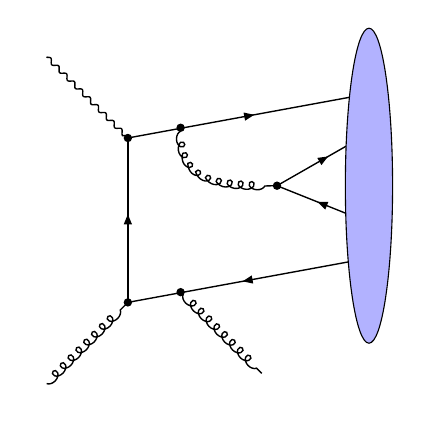
\begin{tikzpicture}
    \begin{feynhand}
  \node (root) at (0,0) {};
  \begin{scope}[on background layer]
    \vertex[dot] (vert1) at (root) {};
    \vertex[dot] (vert2) [below = 2 of vert1] {};

    \vertex[dot](vert3) [above right = .5 and 3 of vert1] {};
    \vertex[dot](vert4) [below = 2 of vert3] {};
    \vertex[dot](vert5) [below left = .37 and 2.33 of vert3]{};
    \vertex[dot](vert6) [below left = .37 and 2.33 of vert4]{};

    \node(dot1) [above left = of vert1] {};
    \node(dot2) [below left = of vert2] {};
    \node(pivot) [below = 1 of vert3] {};
    \node(dot3) [below right = of vert6] {};
    
    \vertex[dot] (split) [left = 1 of pivot] {};
    \vertex[dot] (splitup) [above = .5 of pivot] {};
    \vertex[dot] (splitdown) [below = .3 of pivot] {};

    \propag[pho] (dot1) to (vert1);
    \propag[glu] (dot2) to (vert2);
    \propag[antfer] (vert1) to (vert2);
    \propag[fer] (vert1) to (vert3);
    \propag[antfer] (vert2) to (vert4);
    \propag[glu] (vert5) to [out=270, in=180, looseness=1.2] (split);
    \propag[fer] (split) to (splitup);
    \propag[antfer] (split) to (splitdown);
    \propag[glu] (vert6) to (dot3);
  \end{scope}
  
  \filldraw[fill=blue!30!white] to (pivot) ellipse (.3cm and 2cm);
\end{feynhand}


  \end{tikzpicture}
\end{figure}

\begin{figure}[htb!]
  \centering
  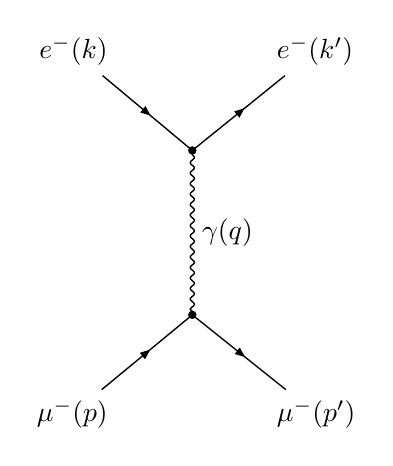
\begin{tikzpicture}
    % --------------------------------------------- %
% electron-muon scattering
% --------------------------------------------- %
\begin{feynhand}
  \vertex[dot] (v1) {};
  \node[dot] (v2) [below=2cm of v1] {};
  \node (e_in) [above left=1.3cm of v1] {$e^{-}(k)$};
  \node (e_out) [above right=1.3cm of v1] {$e^{-}(k^{\prime})$};
  \node (m_in) [below left=1.3cm of v2] {$\mu^{-}(p)$};
  \node (m_out) [below right=1.3cm of v2] {$\mu^{-}(p^{\prime})$};

  \propag[pho] (v1) to [edge label =$\gamma(q)$] (v2);
  \propag[fer] (e_in) to (v1);
  \propag[antfer] (e_out) to (v1);
  \propag[fer] (m_in) to (v2);
  \propag[antfer] (m_out) to (v2);
\end{feynhand}

  \end{tikzpicture}
\end{figure}

\vspace{10pt}

% --------------------------------------------- %
\bibliographystyle{acm}
\bibliography{referencias}
% --------------------------------------------- %
\end{document}


